% This file was created by matlab2tikz.
%
%The latest updates can be retrieved from
%  http://www.mathworks.com/matlabcentral/fileexchange/22022-matlab2tikz-matlab2tikz
%where you can also make suggestions and rate matlab2tikz.
%
\definecolor{mycolor1}{rgb}{0.00000,0.44700,0.74100}%
\definecolor{mycolor2}{rgb}{0.92900,0.69400,0.12500}%
\definecolor{mycolor3}{rgb}{0.46600,0.67400,0.18800}%
\definecolor{mycolor4}{rgb}{0.63500,0.07800,0.18400}%
\definecolor{mycolor5}{rgb}{0.85000,0.32500,0.09800}%
%
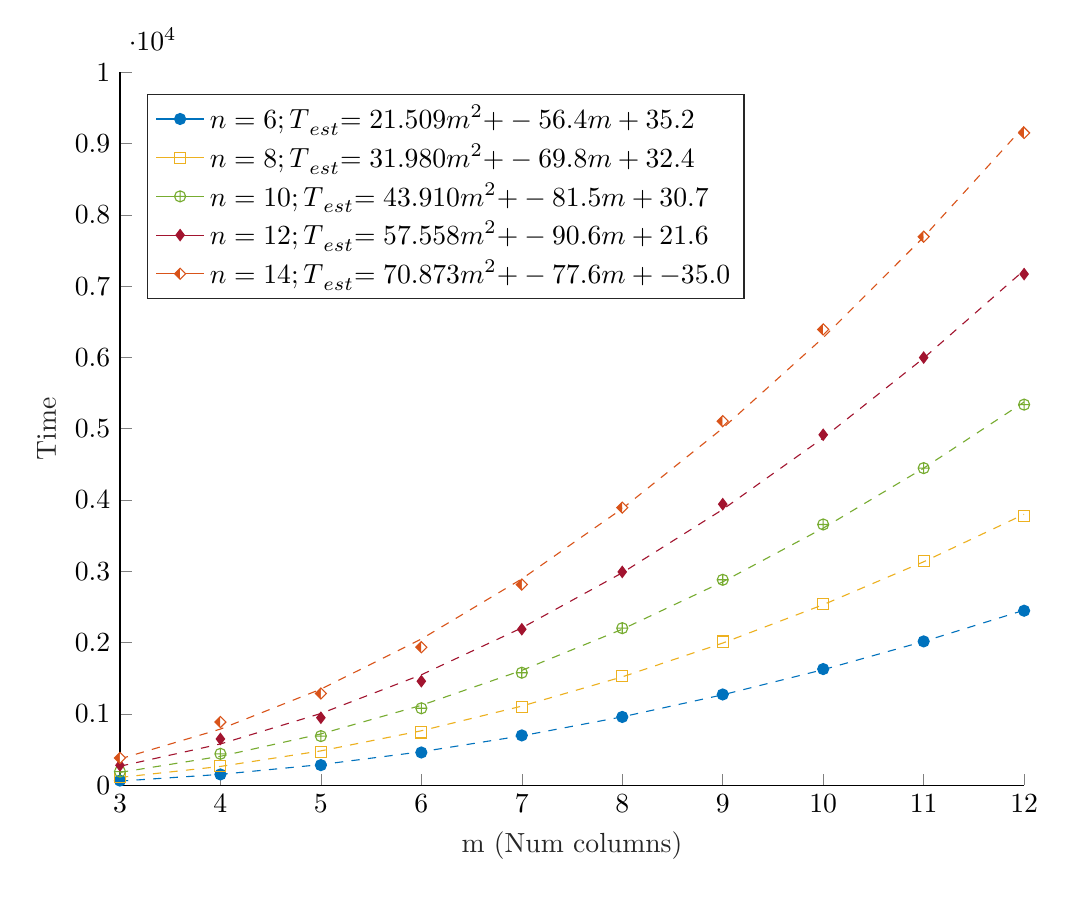
\begin{tikzpicture}

\begin{axis}[%
width=4.521in,
height=3.566in,
at={(0.758in,0.481in)},
scale only axis,
xmin=3,
xmax=12,
xlabel style={font=\color{white!15!black}},
xlabel={m (Num columns)},
ymin=0,
ymax=10000,
ylabel style={font=\color{white!15!black}},
ylabel={Time},
axis background/.style={fill=white},
title style={font=\bfseries},
% title={$\text{Average ticks until solution as a function of m. On n }\times\text{ m grid. (k = 3)}$},
axis x line*=bottom,
axis y line*=left,
legend style={at={(0.03,0.97)}, anchor=north west, legend cell align=left, align=left, draw=white!15!black}
]
\addplot [color=mycolor1, draw=none, mark=*, mark options={solid, mycolor1}]
  table[row sep=crcr]{%
3	66.66\\
4	153.096\\
5	283.422\\
6	460.628\\
7	699.97\\
8	959.118\\
9	1274.124\\
10	1630.398\\
11	2018.254\\
12	2448.368\\
};
\addlegendentry{$\text{n =  6; T}_{\text{est}}\text{ = 21.509m}^\text{2}\text{ + -56.4m +  35.2}$}

\addplot [color=mycolor1, dashed, forget plot]
  table[row sep=crcr]{%
3	59.5330545454505\\
4	153.677260606059\\
5	290.839951515152\\
6	471.021127272729\\
7	694.220787878791\\
8	960.438933333336\\
9	1269.67556363637\\
10	1621.93067878788\\
11	2017.20427878788\\
12	2455.49636363636\\
};
\addplot [color=mycolor2, draw=none, mark=square, mark options={solid, mycolor2}]
  table[row sep=crcr]{%
3	120.096\\
4	274.826\\
5	470.188\\
6	741.584\\
7	1102.424\\
8	1527.888\\
9	2015.708\\
10	2540.05\\
11	3146.168\\
12	3780.586\\
};
\addlegendentry{$\text{n =  8; T}_{\text{est}}\text{ = 31.980m}^\text{2}\text{ + -69.8m +  32.4}$}

\addplot [color=mycolor2, dashed, forget plot]
  table[row sep=crcr]{%
3	110.958527272737\\
4	265.063739393943\\
5	483.128936363636\\
6	765.154118181815\\
7	1111.13928484848\\
8	1521.08443636363\\
9	1994.98957272727\\
10	2532.85469393939\\
11	3134.6798\\
12	3800.4648909091\\
};
\addplot [color=mycolor3, draw=none, mark=oplus, mark options={solid, mycolor3}]
  table[row sep=crcr]{%
3	191.742\\
4	442.14\\
5	690.392\\
6	1080.424\\
7	1579.256\\
8	2203.72\\
9	2882.014\\
10	3657.694\\
11	4447.706\\
12	5338.234\\
};
\addlegendentry{$\text{n = 10; T}_{\text{est}}\text{ = 43.910m}^\text{2}\text{ + -81.5m +  30.7}$}

\addplot [color=mycolor3, dashed, forget plot]
  table[row sep=crcr]{%
3	181.257818181818\\
4	407.0876\\
5	720.737412121212\\
6	1122.20725454545\\
7	1611.49712727273\\
8	2188.60703030303\\
9	2853.53696363636\\
10	3606.28692727273\\
11	4446.85692121212\\
12	5375.24694545455\\
};
\addplot [color=mycolor4, draw=none, mark=diamond*, mark options={solid, mycolor4}]
  table[row sep=crcr]{%
3	281.08\\
4	650.48\\
5	947.736\\
6	1460.034\\
7	2188.854\\
8	2992.5\\
9	3942.424\\
10	4915.346\\
11	5997.69\\
12	7168.05\\
};
\addlegendentry{$\text{n = 12; T}_{\text{est}}\text{ = 57.558m}^\text{2}\text{ + -90.6m +  21.6}$}

\addplot [color=mycolor4, dashed, forget plot]
  table[row sep=crcr]{%
3	267.783418181847\\
4	580.061151515164\\
5	1007.4544\\
6	1549.96316363635\\
7	2207.58744242423\\
8	2980.32723636362\\
9	3868.18254545453\\
10	4871.15336969696\\
11	5989.23970909091\\
12	7222.44156363638\\
};
\addplot [color=mycolor5, draw=none, mark=halfsquare left*, mark options={solid, mycolor5}]
  table[row sep=crcr]{%
3	384.678\\
4	887.814\\
5	1287.79\\
6	1936.76\\
7	2815.5\\
8	3893.6\\
9	5105.982\\
10	6392.258\\
11	7692.926\\
12	9147.614\\
};
\addlegendentry{$\text{n = 14; T}_{\text{est}}\text{ = 70.873m}^\text{2}\text{ + -77.6m + -35.0}$}

\addplot [color=mycolor5, dashed, forget plot]
  table[row sep=crcr]{%
3	370.145363636375\\
4	788.675812121217\\
5	1348.95291212121\\
6	2050.97666363636\\
7	2894.74706666666\\
8	3880.26412121212\\
9	5007.52782727272\\
10	6276.53818484848\\
11	7687.2951939394\\
12	9239.79885454546\\
};
\end{axis}
\end{tikzpicture}%
